\documentclass[10pt]{article}

\usepackage{geometry}
\geometry{margin = 2em, left=2.5cm, top =6em, headheight=\paperheight}
\usepackage[export]{adjustbox}
\usepackage{array}
\usepackage{amsmath}
\usepackage{amsfonts}
\usepackage{fancyhdr}
\pagestyle{fancy}
\fancyhf{}
\lhead{Algebra II}
\chead{Function  Characteristics - Increasing and Decreasing}
\rhead{Action Opportunity A, Page \thepage}
\usepackage{lastpage}
\usepackage{xcolor}
\usepackage{enumitem}
\usepackage{pifont}
\usepackage{graphicx}
\graphicspath{{../img}}
\usepackage{pgfplots}
\pgfplotsset{compat=1.18}
\usepackage{tabularx}

\newcommand{\R}{\mathbb R}
\newcommand{\e}{{\rm e}}
\newcommand{\pobr}[1]{\left\langle#1\right\rangle}
\newcommand{\norm}[1]{\lVert #1 \rVert}
\newcommand{\abs}[1]{\lvert #1 \rvert}

\DeclareMathOperator{\xd}{d\!}
\DeclareMathOperator{\proj}{proj}

\title{}
\date{}

\begin{document}
\noindent
{\large
Last Name \rule{6em}{.1pt}\hspace{\stretch{1}}First Name \rule{6em}{.1pt}\hspace{\stretch{1}} Date \rule{1.5em}{.1pt} -- \rule{1.5em}{.1pt} -- \rule{1.5em}{.1pt}\hspace{\stretch{1}} Period \rule{2em}{.1pt}\hspace{\stretch{1}} Score \rule{2em}{.1pt}
}
\vspace{1em}

\begingroup
\renewcommand{\arraystretch}{1.5}
\begin{center}
\tiny
{
\begin{tabularx}{\textwidth}{|X|X|X|X|X|X|}
\hline
\bf BE PRECISE & \centerline{Integrating} & \centerline{Applying} & \centerline{Practicing} & \centerline{Acquiring} & \centerline{Awaiting Evidence} \\
\hline
I can calculate accurately and efficiently, and be precise in all of my math.&
Selects and applies the correct procedure and solves all routine AND integrating problems.

AND

Expresses the answer to the correct level of precision needed for the problem (including the correct rounding, units, math symbols, labeling, graphing, vocab…)
&Selects and applies the correct procedure and solves all routine problems.


AND

Expresses the answer to the correct level of precision needed for the problem (including the correct rounding, units, math symbols, labeling, graphing, vocab…)
&Selects and applies the correct procedure and solves most routine problems.


AND

Expresses the answer to the correct level of precision needed for the problem (including the correct rounding, units, math symbols, labeling, graphing, vocab…)
&Selects and applies the correct procedure and solves some routine problems.


AND

Attempts to express the answer to the correct level of precision needed for the problem (including the correct rounding, units, math symbols, labeling, graphing, vocab…).
&Selects and attempts to apply the correct procedure for some routine problems.\\
\hline
\bf Criteria&\multicolumn{5}{l|}{\parbox[c][4em]{.8\textwidth}{}}\\
\hline
\end{tabularx}
}
\end{center}
\endgroup
\vspace{1em}

\footnotesize
\begin{enumerate}
\item Use the following symbols to label the correspondent elements of the graph.

\begin{center}
\Large
\fbox{
\begin{tabular}{ll}
$\bigcirc$ : $x-$intercept/zeros & $\square$ : $y-$intercept\\
$\triangle$ :  relative maximum & $\lvert\triangle\rvert$ :  absolute maximum\\
$\nabla$ : relative minimum & $\lvert\nabla\rvert$ : absolute minimum\\
\ \begin{tikzpicture}
\draw[dash dot] (0,0) -- (0,1);
\end{tikzpicture}\hspace{.5em}: vertical axis of symmetry
\end{tabular}}
\vspace{1em}

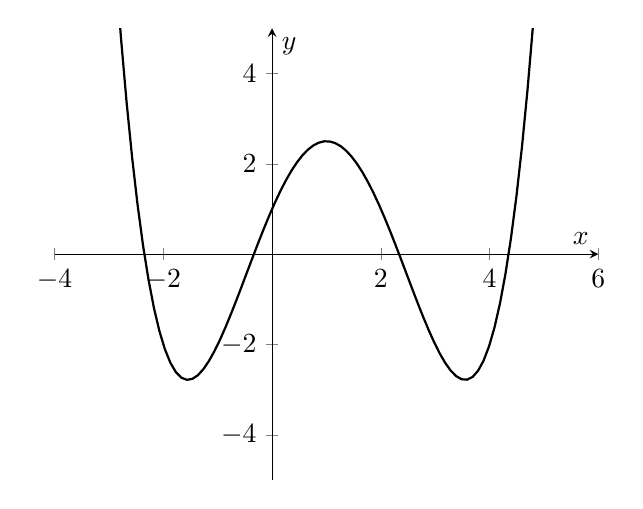
\begin{tikzpicture}
\begin{axis}[
    xlabel={$x$},
    ylabel={$y$},
    axis lines=middle,
    xmin=-4,xmax=6,
    ymin=-5,ymax=5,
    domain=-5:5,
    samples=100,
    width=0.7\textwidth
]
\addplot[thick]{(x-1+3)*(x-1+2)*(x-1-2)*(x-1-3)/8-2};
\end{axis}
\end{tikzpicture}

\end{center}
\item Consider the interval $[-2,3]$.
\begin{enumerate}
\item Shade the segment represented by the interval above on the number line.
\vspace{1em}
\begin{center}
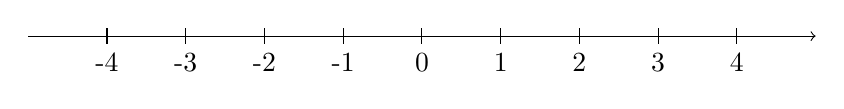
\begin{tikzpicture}
  \draw[->] (-5,0) -- (5,0);
  \foreach \x in {-4,..., 4}
    \draw (\x,0.1) -- (\x,-0.1) node[below] {\x};
\end{tikzpicture}
\end{center}
\vspace{2em}
\item Write the interval as an inequality. \rule{12em}{0.1pt}
\clearpage

\end{enumerate}
\item The following chart summarizes the New York house price index in 2021 through 2025.
\begin{figure}[h]
\centering
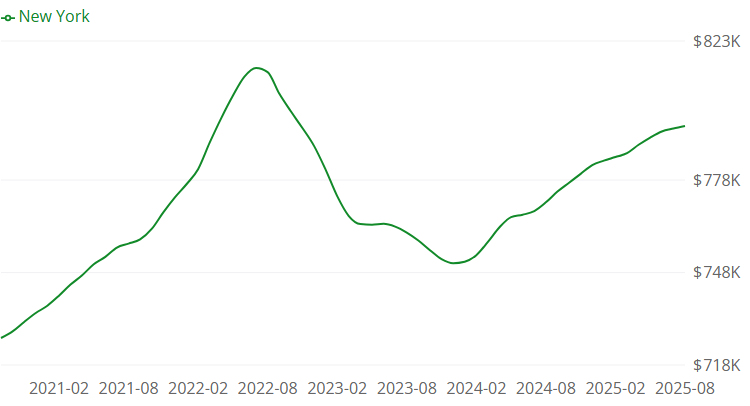
\includegraphics[width=.6\textwidth]{new-york-house-price-2021-2025.png}
\end{figure}

\begin{enumerate}
\item
Identify the period(s) when the housing prices were decreasing. \rule{12em}{.1pt}\\[1.5em]
\item
Estimate the net loss over the decreasing period you identified above. \rule{12em}{.1pt}
\end{enumerate}

\item
List the turning points, and then use the points to write what intervals it’s
increasing and decreasing from.
\begin{center}
\begin{tabular}{p{0.5\textwidth}p{0.5\textwidth}}
\parbox{0.5\textwidth}{
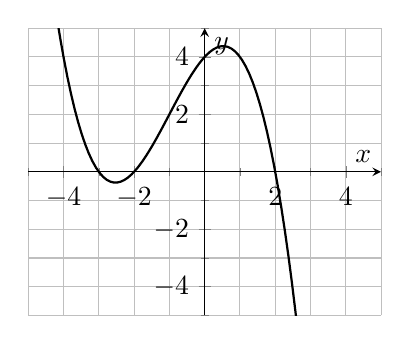
\begin{tikzpicture}
\begin{axis}[
    xlabel={$x$},
    ylabel={$y$},
    grid=both,
    minor tick num=1,
    axis lines=middle,
    xmin=-5,xmax=5,
    ymin=-5,ymax=5,
    domain=-5:5,
    samples=100,
    width=0.5\textwidth
]
\addplot[thick]{-(x+3)*(x+2)*(x-2)/3};
\end{axis}
\end{tikzpicture}
}&\parbox[c]{0.5\textwidth}{
\begin{itemize}[leftmargin=0em]
\item
{\bf Turning Points}\\[1em]
\rule{0.4\textwidth}{0.5pt}\\[1em]
\rule{0.4\textwidth}{0.5pt}\\[1em]
\rule{0.4\textwidth}{0.5pt}
\item
{\bf Increasing Intervals}\\[1em]
\rule{0.4\textwidth}{0.5pt}\\[1em]
\rule{0.4\textwidth}{0.5pt}\\[1em]
\rule{0.4\textwidth}{0.5pt}
\item
{\bf Decreasing Intervals}\\[1em]
\rule{0.4\textwidth}{0.5pt}\\[1em]
\rule{0.4\textwidth}{0.5pt}\\[1em]
\rule{0.4\textwidth}{0.5pt}
\end{itemize}
}
\end{tabular}
\end{center}
\item
List the turning points, and then use the points to write what intervals it’s
increasing and decreasing from.

\begin{center}
\begin{tabular}{p{0.5\textwidth}p{0.5\textwidth}}
\parbox{0.5\textwidth}{
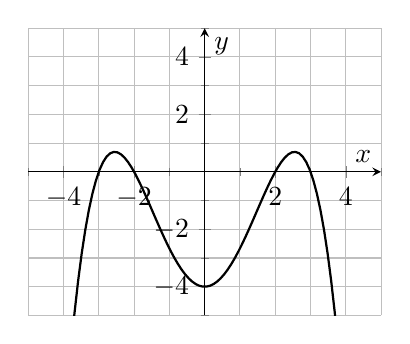
\begin{tikzpicture}
\begin{axis}[
    xlabel={$x$},
    ylabel={$y$},
    grid=both,
    minor tick num=1,
    axis lines=middle,
    xmin=-5,xmax=5,
    ymin=-5,ymax=5,
    domain=-5:5,
    samples=100,
    width=0.5\textwidth
]
\addplot[thick]{-(x+3)*(x+2)*(x-2)*(x-3)/9};
\end{axis}
\end{tikzpicture}
}&\parbox[c]{0.5\textwidth}{
\begin{itemize}[leftmargin=0em]
\item
{\bf Turning Points}\\[1em]
\rule{0.4\textwidth}{0.5pt}\\[1em]
\rule{0.4\textwidth}{0.5pt}\\[1em]
\rule{0.4\textwidth}{0.5pt}
\item
{\bf Increasing Intervals}\\[1em]
\rule{0.4\textwidth}{0.5pt}\\[1em]
\rule{0.4\textwidth}{0.5pt}\\[1em]
\rule{0.4\textwidth}{0.5pt}
\item
{\bf Decreasing Intervals}\\[1em]
\rule{0.4\textwidth}{0.5pt}\\[1em]
\rule{0.4\textwidth}{0.5pt}\\[1em]
\rule{0.4\textwidth}{0.5pt}
\end{itemize}
}
\end{tabular}
\end{center}
\end{enumerate}
\end{document}